%//------ Section 03 -------------------------------------------------------------------------------------------------
\chapter{Introduction}
\label{appendix:ExtendedAbstractFrench}
%//-----------------------------------------------------------------------//

Tous les phénomènes observés dans la Nature peuvent actuellement être décrits par quatre interactions fondamentales : les interactions gravitationnelles, électromagnétiques, fortes et faibles. La compréhension de ces forces a été au cœur de la recherche en physique tout au long des \upperRomannumeral{19}$^{\textrm{e}}$ et \upperRomannumeral{20}$^{\textrm{e}}$ siècles. Cela a conduit aux deux piliers de la physique moderne : la théorie de la relativité générale d'Einstein, dans laquelle la gravité est un effet géométrique de la topologie -- en particulier, de la courbure -- de l'espace-temps, et le Modèle Standard de la physique des particules. Dans ce dernier cas, les trois autres forces sont comprises comme un échange de particules élémentaires (bosons vecteurs de jauge ou quanta) de leur champ quantique sous-jacent.

Dans le cadre du Modèle Standard, l'interaction forte est décrite par la chromodynamique quantique (\textbf{Q}uantum \textbf{C}hromo\textbf{D}ynamics, QCD). Dans cette théorie, les \textit{quarks} -- les particules élémentaires sensibles à cette force -- portent une charge de \textit{couleur}\footnote{C'est l'analogue de la charge électrique en QCD.}, ce qui permet l'échange de \textit{gluons}, les bosons vecteurs de jauge de la QCD. La particularité de cette théorie réside dans sa structure non-abélienne, ce qui signifie que les gluons eux-mêmes ont une charge de couleur et peuvent donc interagir entre eux. La conséquence directe de cette caractéristique est la variation de la constante de couplage QCD avec l'échelle d'énergie. Dans les processus impliquant d'importants transferts d'impulsion (ou à faible distance), la constante de couplage s'affaiblit et les partons -- quarks et gluons -- peuvent être considérés comme des particules libres : c'est la liberté asymptotique. En revanche, pour des faibles échanges d'impulsion (ou à une plus grande distance, typiquement de l'ordre de la taille du proton), le couplage augmente, obligeant les partons à être confinés à l'intérieur d'objets composites, appelés \textit{hadrons}, constitués généralement de deux ou trois quarks de valence : les \textit{mésons} et les \textit{baryons} respectivement. Dans ce régime, les calculs de la QCD ne peuvent être réalisés que par des approches non-perturbatives. L'une de ces approches révèle une autre caractéristique intéressante : la  \textit{lattice QCD} (lQCD) prédit une transition de phase de la matière hadronique à la matière partonique à des températures et/ou densités extrêmement élevées ; étant donné que les partons sont déconfinés et que l'on pensait qu'ils interagissaient faiblement -- de manière similaire aux plasmas --, cet état de la matière a été appelé \say{plasma quark-gluon} ou \say{\textit{quark-gluon plasma}} (QGP). Celui-ci correspond supposément à l'état de l'Univers primordial, pendant les premières microsecondes de son existence, et pourrait être présent encore de nos jours à une échelle macroscopique dans le noyau des étoiles à neutrons.\\

Le QGP n'est pas seulement un concept, il est désormais un fait expérimental. Bien que les premières études remontent aux années 1970, la recherche sur le QGP a pris un tournant en 2000 avec les premiers signes de son existence observés par les expériences du programme d'ions lourds du CERN (Organisation européenne pour la recherche nucléaire) \cite{cernNewStateMatter2023}. Cela a été confirmé plus tard en 2005 par les quatre expériences du \textit{Relativistic Heavy-Ion Collider} (Brookhaven National Laboratory) avec leurs \textit{livres blancs} respectifs \cite{ludlamHUNTINGQUARKGLUON2005, arseneQuarkGluonPlasma2005, backPHOBOSPerspectiveDiscoveries2005, phenixcollaborationFormationDensePartonic2005, starcollaborationExperimentalTheoreticalChallenges2005}.

Expérimentalement, le QGP est reproduit en laboratoire en faisant entrer en collision des noyaux lourds (Xe, Au, Pb, ...) à des énergies extrêmement élevées. En raison de sa courte existence d'environ $10^{-23}$ seconde, l'étude de cet état exotique de la matière repose principalement sur l'observation des traces/signatures laissées après la collision. L'exploration du QGP repose également sur des collisions plus élémentaires, notamment les collisions proton-noyau et proton-proton (pp), où aucun QGP n'est anticipé \textit{a priori} et qui sont donc utilisées comme références.

Parmi les différentes sondes disponibles du QGP, les baryons multi-étranges, \rmXi et \rmOmega, contenant deux ou trois quarks \textit{étranges}, jouent un rôle particulier. Étant situés entre les particules légères et lourdes du point de vue de la saveur, ils constituent des hadrons non-ordinaires produits en abondance lors de collisions à haute énergie, ce qui fournit des contraintes efficaces pour les modèles statistiques. De plus, grâce à une topologie de désintégration caractéristique (cascade), leur identification est possible sur un vaste domaine d'impulsion transverse, associé à différents mécanismes de production (éventuellement entrelacés). Enfin, une signature clé du QGP est \textit{l'enrichissement en étrangeté}, qui se traduit par une augmentation de la production de quarks étranges et, par conséquent, dans l'état final, de hadrons étranges. En particulier, cet enrichissement s'intensifie pour les hadrons ayant une grande teneur en étrangeté, à savoir les \rmXi et les \rmOmega.\\

Aujourd'hui, l'expérience au CERN consacrée à l'étude de la QCD et du QGP est \textit{A Large Ion Collider Experiment} (ALICE), installée sur l'anneau du Grand Collisionneur d'Hadron (\textit{Large Hadron Collider}, LHC). Après deux campagnes de prise de données en 2009-2013 (Run-1) et 2015-2018 (Run-2), le LHC a redémarré le 5 juillet 2022 pour un programme de quatre ans (Run-3) \cite{cernThirdRunLarge2023}. Pendant la deuxième longue période d'arrêt du collisionneur (2018-2022), ALICE a été entièrement modernisée et ré-émerge flambant neuve : un trajectographe interne (\textit{Inner Tracking System}) plus précis avec un budget de matière réduit ; une lecture améliorée pour sa chambre à projection temporelle (\textit{Time Projection Chamber})~; l'installation d'un trajectographe à muons à rapidité à l'avant (\textit{Muon Forward Tracker}) ; des détecteurs améliorés, associés à un nouveau logiciel dit \textit{online-offline} pour permettre une lecture continue, permettant un enregistrement des collisions Pb-Pb pour des taux d'intéraction atteignant 50 kHz et typiquement 500 kHz pour des collisions pp~\cite{alicecollaborationUpgradeALICEExperiment2014}. Grâce à ces améliorations, l'étude de la QCD et du QGP au LHC entre dans une nouvelle ère, un âge de \say{précision}.

En ce qui concerne la précision, il est éclairant de se demander ce que cela signifie vraiment ; après tout, personne ne réalise des mesures imprécises. Dans le contexte actuel, cela englobe deux aspects : d'une part, une exploration/caractérisation approfondie de l'objet d'étude avec de nouvelles observables ou des mesures précédemment impossibles maintenant à portée de main ; d'autre part, des mesures précises allant bien au-delà des limites statistiques ou systématiques actuelles. À cet égard, en examinant les mesures des précédentes campagnes de prise de données, à savoir du LHC Run-1 et Run-2, il existe, dans une certaine mesure, de nombreuses mesures précises, notamment dans le secteur des saveurs légères. Par exemple, nous pouvons mentionner \cite{alicecollaborationProductionLambdaOverline2023, alicecollaborationMeasurementLifetimeMathrm2023, ciaccoEasuringMuLHC2023, alicecollaborationCharacterizingInitialConditions2022, schotterMultidifferentialInvestigationStrangeness2023, schotterQCDLHC20222022}.\\

Cette thèse propose de poursuivre cet effort de précision sur les baryons multi-étranges grâce aux excellentes capacités de trajectographie et d'identification à rapidité centrale d'ALICE lors du LHC Run-2. L'accent est mis sur les collisions pp à une énergie dans le centre de masse de \sqrtS = 13 TeV. Au cours de ces trois années de thèse s'étalant de 2020 à 2023, deux analyses ont été réalisées.

\chapter{Mesures de masse des baryons multi-étranges dans les collisions pp à \sqrtS = 13 TeV}

La première analyse réalisée au cours de cette thèse vise à mesurer les masses et les différences de masse entre particule et anti-particule. Cette mesure se concentre sur les baryons multi-étranges, à savoir les \rmXiM, \rmAxiP, \rmOmegaM et \rmAomegaP.\\

Le Modèle Standard repose sur un ensemble de symétries, chacune étant soit discrète -- comme la combinaison de la conjugaison de charge (C), de la parité (P) et de l'inversion du temps (T), connue sous le nom de transformation CPT -- soit continue -- par exemple, les transformations de Lorentz qui incluent les rotations et les \textit{boosts}. En particulier, les symétries de Lorentz et CPT sont liées par le théorème CPT qui établit que toute théorie quantique des champs unitaire, locale et invariante de Lorentz doit également être invariante sous la transformation CPT \cite{kosteleckyStatusCPT1998}. Par conséquent, la violation de la symétrie CPT impliquerait la rupture de la symétrie de Lorentz, et vice versa\footnote{En fait, il existe une autre option ; pour permettre la violation de la symétrie CPT, soit la symétrie de Lorentz doit être brisée -- comme en théorie des cordes \cite{kosteleckySpontaneousBreakingLorentz1989} ou dans l'extension du Modèle Standard (\textit{Standard-Model Extension}) \cite{colladayLorentzviolatingExtensionStandard1998} -- soit certaines des autres hypothèses du théorème CPT doivent être abandonnées, à savoir la positivité de l'énergie \cite{abersDiseasesInfiniteComponentField1967}, les interactions locales \cite{carruthersIsospinSymmetryTCP1968}, le spin fini \cite{oksakInvalidityTCPtheoremInfinitecomponent1968}, etc \cite{lehnertCPTSymmetryIts2016, greenbergCPTViolationImplies2002}.} \cite{sozziTestsDiscreteSymmetries2019}. Une autre implication concerne la relation entre les propriétés de la matière et de l'antimatière : en raison de la conjugaison de charge liant les particules aux antiparticules, la symétrie CPT impose qu'elles partagent la même masse invariante, les mêmes spectres de masse, la même durée de vie, les mêmes constantes de couplage, etc \cite{lehnertCPTSymmetryIts2016}. La plupart des vérifications expérimentales de l'invariance CPT découlent de ce dernier point, ce qui impose plusieurs contraintes sur les propriétés des antiparticules.\\

Le \textit{Particle Data Group}\footnote{Il s'agit d'une collaboration internationale de physiciens visant à : i) compiler et ré-analyser les publications relatives aux propriétés fondamentales des particules en vue de fournir les valeurs les plus précises (en présentant les mesures atteignant la plus haute précision ou le cas échéant, en calculant la moyenne des mesures mondiales) ; ii) présenter l'état de l'art de la physique des particules et de la cosmologie.} (PDG) \cite{particledatagroupReviewParticlePhysics2022} compile une grande variété de tests de la symétrie CPT réalisés dans de nombreuses expériences et avec différents degrés de précision ; jusqu'à présent, aucune violation de la symétrie CPT n'a été observée. Le test le plus contraignant implique l'oscillation des \rmKzero-\rmAKzero, qui dépend de la différence de masse et de durée de vie entre ces deux états. De cette manière, en supposant qu'il n'y ait pas d'autre source de violation de la symétrie CPT dans la désintégration des kaons neutres, ces deux quantités ont été bornées \cite{particledatagroupReviewParticlePhysics2022, angelopoulosK0OverlineK1999} à

\begin{equation}
2 \frac{\mid m_{\rmKzero} - m_{\rmAKzero} \mid}{m_{\rmKzero} + m_{\rmAKzero}} < 6 \times 10^{-19} \quad , \quad 2 \frac{\mid \Gamma_{\rmKzero} - \Gamma_{\rmAKzero} \mid}{\Gamma_{\rmKzero} + \Gamma_{\rmAKzero}} = (8 \pm 8) \times 10^{-18}.
\end{equation}

Ces limites indirectes sont beaucoup plus contraignantes que celles typiquement extraites avec des tests directs. Par exemple, dans le secteur des hypérons, la précision sur la différence de masse relative est généralement de l'ordre de quelques $10^{-5}$. Dans ce dernier cas, il convient de mentionner qu'il existe encore des possibilités d'amélioration, en particulier en ce qui concerne les mesures des différences de masse entre particules et anti-particules dans le secteur des baryons multi-étranges. Le seul test de cette nature remonte à 2006 \cite{abdallahMassesLifetimesProduction2006} pour les \rmXiM et \rmAxiP, et à 1998 \cite{chanMeasurementPropertiesOverline1998} pour les \rmOmegaM et \rmAomegaP. Le premier a été réalisé en exploitant les désintégrations hadroniques de 3,25 millions de \rmZzero enregistrées par le détecteur DELPHI au LEP-1 ; le second a été obtenu avec le spectromètre E756 à Fermilab, en utilisant un faisceau de protons de 800 \gmom sur une cible de béryllium. Cependant, les deux études souffrent d'une faible statistique : environ 2500(2300) \rmXiM (\rmAxiP) reconstruits et environ 6323(2607) \rmOmegaM (\rmAomegaP) reconstruits ont été utilisés.\\

\begin{table}[t]
    \centering
    \begin{tabular}{>{\centering\arraybackslash}b{1.5cm}@{\hspace{0.3cm}} >{\centering\arraybackslash}b{1.75cm}@{\hspace{0.3cm}} >{\centering\arraybackslash}b{2.85cm}@{\hspace{0.3cm}} >{\centering\arraybackslash}b{3.6cm}@{\hspace{0.3cm}} >{\centering\arraybackslash}b{2.5cm}@{\hspace{0.3cm}} >{\centering\arraybackslash}b{1cm}@{\hspace{0.3cm}}}
    \noalign{\smallskip}\hline\noalign{\smallskip}
	Particle & Quark content & Mass (\mmass) & Relative mass difference & Dominant decay channel & B.R.\\	
    \noalign{\smallskip}\hline \noalign{\smallskip}
    	
	\rmKzeroS & $d \bar{s}$ & $497.611 \pm 0.013$ & $< 6 \times 10^{-19}$ & \piPlus \piMinus & 69.20\%\\
	
    \noalign{\smallskip}\hline \noalign{\smallskip}
    
    \rmLambda (\rmAlambda) & $u d s$ ($\bar{u}\bar{d}\bar{s}$) & $1115.683 \pm 0.006$ & $\left(-0.1 \pm 1.1\right) \times 10^{-5}$ & \proton \piMinus (\pbar \piPlus) & 63.9\% \\
    
    \noalign{\smallskip}\hline \noalign{\smallskip}    
    
    \rmXiM (\rmAxiP) & $dss$ ($\bar{d}\bar{s}\bar{s}$) & $1321.71 \pm 0.07$ & $\left(-2.5 \pm 8.7\right) \times 10^{-5}$ & \rmLambda \piMinus (\rmAlambda \piPlus) & 99.9\% \\	
    \noalign{\smallskip}\hline \noalign{\smallskip}
    
	\rmOmegaM (\rmAomegaP) & $sss$ ($\bar{s}\bar{s}\bar{s}$) & $1672.45 \pm 0.23$ & $\left(-1.44 \pm 7.98\right) \times 10^{-5}$ & \rmLambda \rmKminus (\rmAlambda \rmKplus) & 67.8\%\\    
    \noalign{\smallskip}\hline\noalign{\smallskip}
    \end{tabular}
    \caption{Quelques caractéristiques des hypérons \rmLambda, \rmXi, \rmOmega et du méson \rmKzeroS en 2023 : contenu en quarks, masse, différence de masse relative avec leurs incertitudes associées, leur canal de désintégration dominant ainsi que le rapport d'embranchement~\cite{particledatagroupReviewParticlePhysics2022}.}\label{tab:V0CascPDGMass}
\end{table}

En comparaison, l'ensemble des collisions pp à une énergie dans le centre de masse de 13 TeV collectées par ALICE tout au long du LHC Run-2 contiennent environ 2 500 000 hypérons \rmXi et 133 000 hypérons \rmOmega, avec un faible bruit de fond. Par conséquent, dans cette thèse, la mesure de la différence de masse entre les hypérons \rmXiM et \rmAxiP, ainsi qu'entre les hypérons \rmOmegaM et \rmAomegaP, est effectuée. Elle repose sur des échantillons de données beaucoup plus importants que ceux précédemment exploités. Ces mesures directes de la différence de masse devraient offrir un test de la symétrie CPT à un niveau de précision sans précédent dans le secteur des baryons multi-étranges. Les valeurs de masse sont également mises à jour, avec une précision sensiblement meilleure que les mesures passées, actuellement répertoriées dans le PDG et utilisées dans le calcul des valeurs moyennes mondiales. Ces dernières sont présentées dans le \tab\ref{tab:V0CascPDGMass}.

De plus, en ce qui concerne l'hypéron \rmLambda et le méson \rmKzeroS, le PDG cite une précision de quelques \kmass sur la valeur de la masse, et d'environ $1 \times 10^{-5}$ sur la valeur de la différence de masse relative\footnote{Cela ne concerne que la différence de masse relative entre le l'hypéron \rmLambda et l'anti-hypéron \rmAlambda. Comme mentionné précédemment, une telle quantité est plus faible de quatorze ordres de grandeur dans le cas du \rmKzeroS.}. Abondamment produits, ces deux hadrons présentent également une caractéristique intéressante dans le contexte de cette thèse~: ils suivent une désintégration en V0 dans leur canal de désintégration dominant, et peuvent donc être identifiés de manière similaire aux cascades en utilisant une reconstruction topologique. Pour ces deux raisons -- une grande précision sur les valeurs de masse du PDG et une topologie de désintégration similaire à celle des cascades --, l'analyse est reproduite sur l'hypéron \rmLambda et le méson \rmKzeroS, tous deux servant de références pour la mesure.\\

Les \rmXi et \rmOmega sont étudiés dans leur canal de désintégration en cascade : $\rmXiPM \rightarrow \rmLambdaPM \rmPiPM \rightarrow \pOrPbar \rmPiPM \rmPiPM$ et $\rmOmegaPM \rightarrow \rmLambdaPM \rmKPM \rightarrow \pOrPbar \rmPiPM \rmKPM$. La reconstruction de cette topologie en cascade passe par l’appariement de trois particules chargées ; l'association de deux particules de charges électriques opposées permet de former un candidat \rmLambda ou \rmAlambda (candidat \textit{V0}), qui peut lui-même associé à une autre particule (particule \textit{célibataire}) pour former un candidate cascade. Dans une collision pp, la densité en particules chargées peut varier de quelques particules jusqu'à une cinquantaine. La simple association de trois particules aboutit nécessairement à la formation de candidats erronés qui, le cas échéant, constituent un bruit de fond combinatoire. Ce dernier est réduit en ayant recours à quatorze sélections topologiques, visant à identifier les combinaisons spatialement compatibles avec la topologie de désintégration attendue. La sélection des candidats \rmXi ou \rmOmega effectuée, leur distribution en masse invariante est reconstruite et ajustée typiquement par la somme de deux fonctions: une triple Gaussienne\footnote{Il s'agit de la somme de trois Gaussiennes centrées autour de la même valeur moyenne avec des variances différentes.} pour le pic de masse invariante et d'une exponentielle pour le bruit de fond. Cette dernière étape permet d’extraire la masse, ainsi que le signal brute des \rmXi ou \rmOmega, telle que représentée sur les \figs\ref{fig:InvMassCascades}.

\begin{figure}[!p]
%\centering
\hspace*{-1.5cm}
\subfigure[]{
	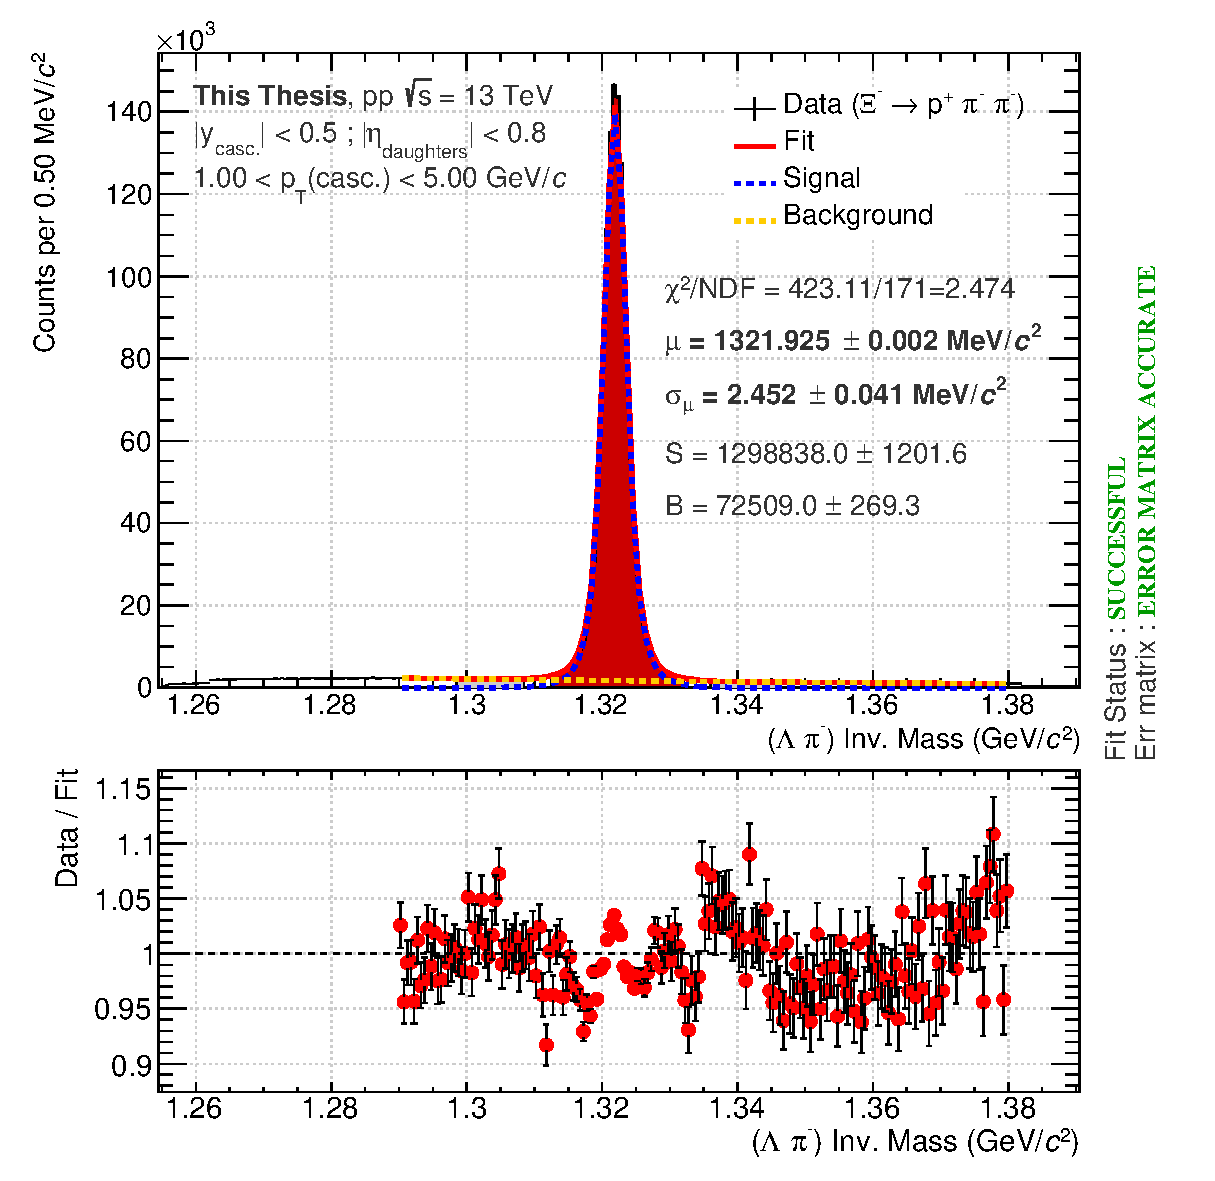
\includegraphics[width=0.6\textwidth]{Figs/Chapter5/InvMassXiMinus.eps}
	\label{fig:XiMinus_TripleGaussian}
} 
\subfigure[]{
	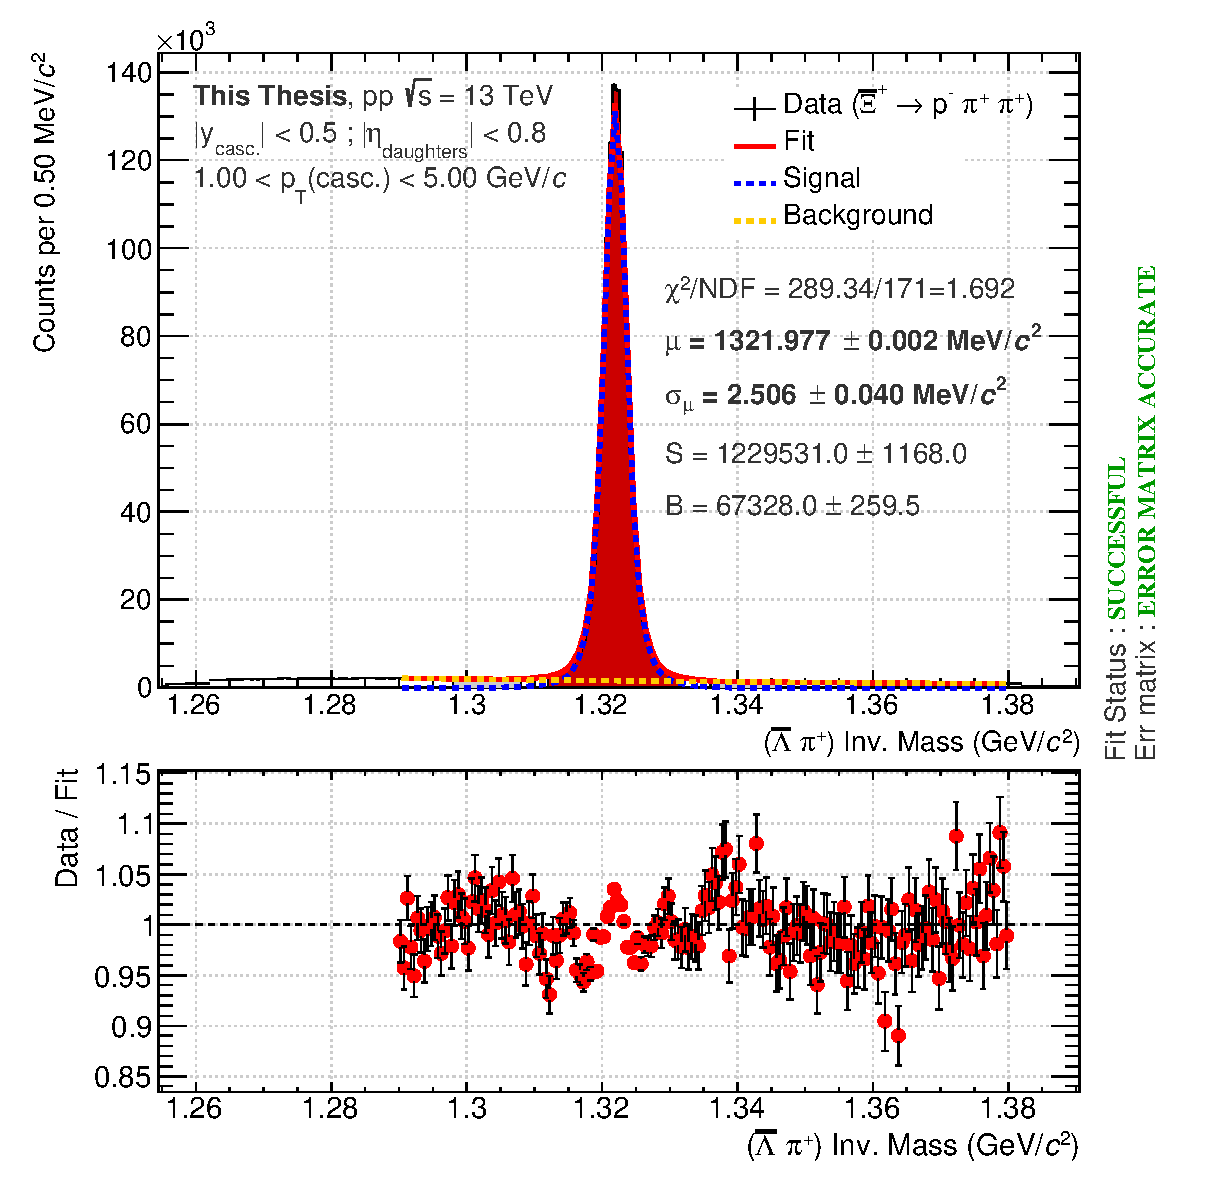
\includegraphics[width=0.6\textwidth]{Figs/Chapter5/InvMassXiPlus.eps}
	\label{fig:XiPlus_TripleGaussian}
} 
\hspace*{-1.5cm}
\subfigure[]{
	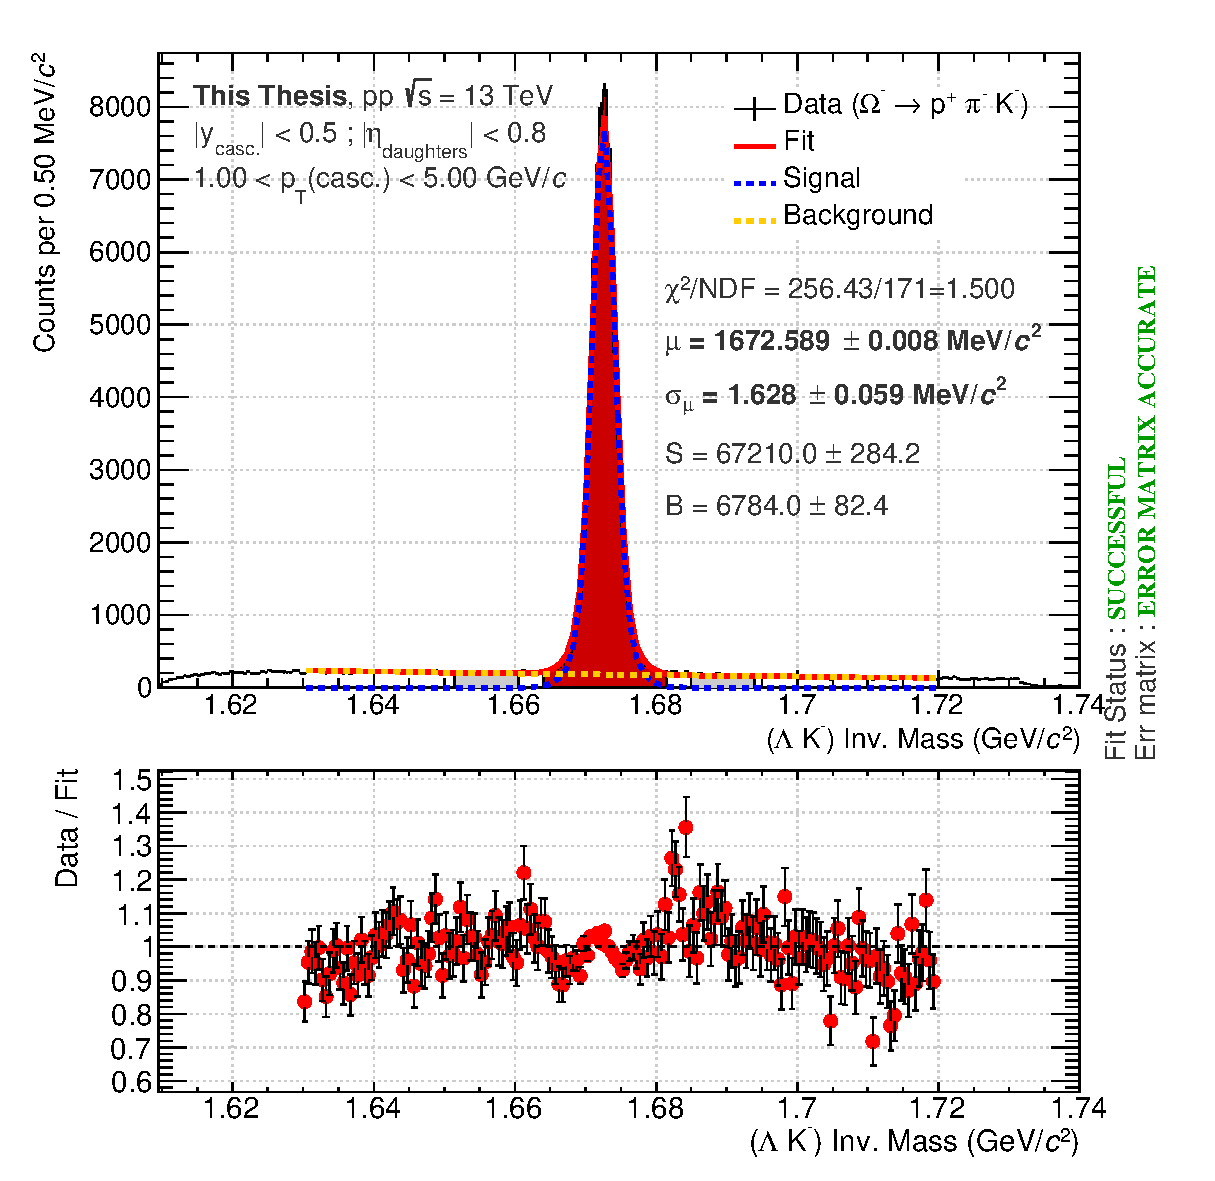
\includegraphics[width=0.6\textwidth]{Figs/Chapter5/InvMassOmegaMinus.eps}
	\label{fig:OmegaMinus_TripleGaussian}
} 
\subfigure[]{
	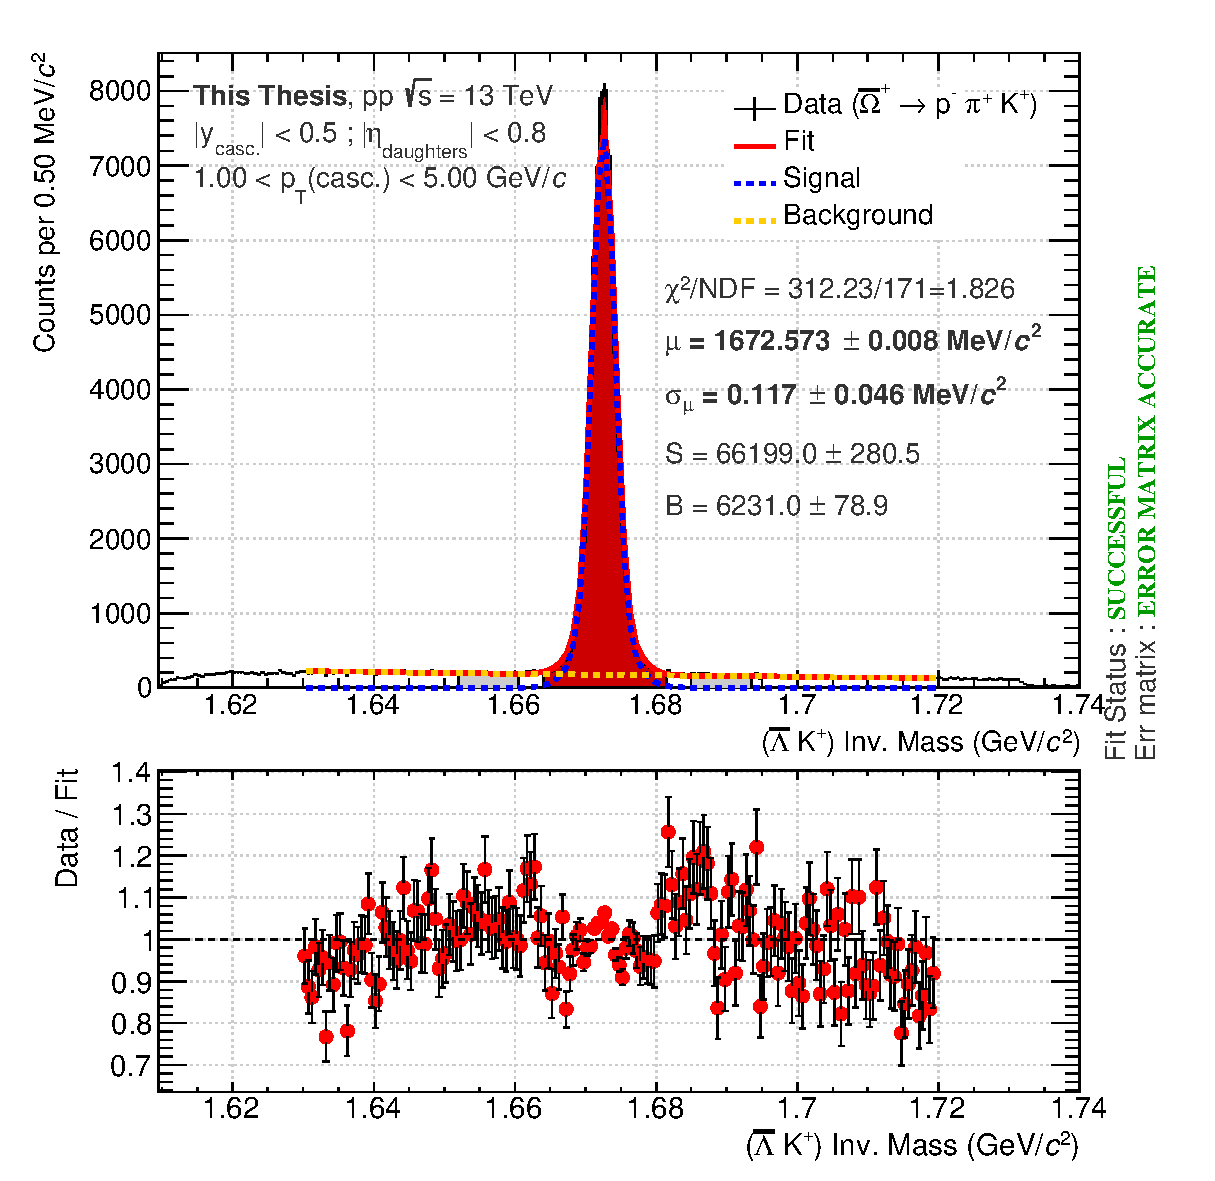
\includegraphics[width=0.6\textwidth]{Figs/Chapter5/InvMassOmegaPlus.eps}
	\label{fig:OmegaPlus_TripleGaussian}
}  
\caption{Distributions de masse invariante des hypérons \rmXiM (a), \rmAxiP (b), \rmOmegaM (c) and \rmAomegaP (d) dans les collisions pp à \sqrtS = 13 \tev. Ici, le pic est modélisé par une triple Gaussienne, et le bruit de fond par une fonction exponentielle. Chaque distribution est accompagné d'une sous-figure représentant l'accord entre les données et le modèle, sous la forme d'un ratio pour chaque entrée de la distribution. Les barres d'erreurs tiennent compte des incertitudes sur ces deux quantités.}
	\label{fig:InvMassCascades}
\end{figure}

Tous les ajustements sont d'une qualité raisonablement satisfaisante. Les paneaux inférieurs montrent que l'écart données-modèle  n'excède pas les 5\% pour les points les plus précis, \ie ceux dans la région du pic. Le pic de masse invariante est assis sur un faible bruit de fond : 1 298 838 $\pm$ 1202 \rmXiM (1 229 531 $\pm$ 1168 \rmAxiP ) et 67~210~$\pm$~285~\rmOmegaM (66 199 $\pm$ 281 \rmAomegaP) ont été reconstruits avec des puretés supérieurs à 90\%.\\

Le c\oe{}ur de cette mesure repose sur la réalisation d’une étude détaillée des incertitudes systématiques associées. De façon générale, la stratégie employée consiste à reprendre l’analyse en variant certaines de ses composantes. Par exemple, l’une des sources d’incertitudes systématiques est liée à la sélection de nos candidats. Pour l’estimer, j’ai implémenté une procédure dans laquelle la sélection des candidats et l’extraction de leur masse sont répétées 20 000 fois avec des valeurs de sélection générées aléatoirement. D’autres sources d’incertitudes systématiques ont été considérées : la précision du champ magnétique, le choix des fonctions et plages d’ajustement, la contribution de l’empilement de collisions dans l’événement, l’influence des incertitudes sur la masse des produits de désintégration (\rmLambda, \rmPiPM, \rmKPM), l’efficacité de reconstruction de la masse. 

Les sources dominantes de biais systématiques proviennent i) des erreurs sur les corrections des pertes en énergie et ii) la calibration imparfaite résiduelle du detecteur ALICE. Les premières peuvent apparaître sous deux aspects. Il y a l’écart entre la quantité de matière connue et celle effectivement traversée par les particules, qui aboutit à une estimation erronée des pertes d’énergie et \textit{in fine} un biais dans la masse mesurée. La seconde trouve ses origines dans certaines approximations réalisées lors de l'implémentation des corrections des pertes d'énergie. Elles sont au nombre de trois, classée de la plus à la moins importantes.
\begin{enumerate}
\item Lors de la dernière étape de reconstruction des traces laissées dans le detecteur par les particules chargées, toutes les traces sont extrapolées à leur point de plus courte approche au vertex primaire, en prenant en compte les différents processus stochastisques tels que celui des pertes d'énergie dans la matière. Bien que cela ait du sens dans le cas d'une particule primaire, cette approche introduit un biais pour les particules dites \textit{secondaires}, issues de la désintégration d'une autre particule comme le \rmKzeroS, \rmLambda, \rmXi ou \rmOmega : pour celles-ci, l'extrapolation devrait s'arrêter au point de désintégration. Au lieu de cela, à chaque étape de la propagation entre le vertex secondaire et primaire, la trace reçoit davantage d'énergie du fait de l'application des corrections des pertes d'énergie. Cet excès d'énergie s'accumule avec la distance du point de désintégration :  plus loin est le vertex secondaire, plus les paramètres des traces associées sont biasées. Néanmoins, à ce stade de la reconstruction, il n'y a aucun moyen de distinguer une particule primaire d'une secondaire. C'est pourquoi ce biais est censé être éliminé plus tard lors de la reconstruction des V0s et des cascades. Cependant, ces reconstructions sont effectuées sans aucune correction des pertes d'énergie. Cela signifie que l'excédent d'énergie précédemment ajoutée durant la propragation entre le vertex secondaire et primaire n'a pas été soustraite, ce qui entraîne un biais sur l'énergie/impulsion des particules au vertex secondaire, et donc sur la masse mesurée des V0s et cascades. 

\item La perte d'énergie linéique moyenne est donnée par la formule de Bethe-Bloch:
\begin{equation}
\begin{split}
\langle -\frac{dE}{dx} \rangle &= K z^{2} \frac{Z}{A} \frac{1}{\beta^{2}} \left[ \frac{1}{2} \ln \frac{2 m_{e} c^{2} \beta^{2} \gamma^{2} T_{\rm max}}{I} - \beta^{2} - \frac{\delta \left( \beta \gamma \right)}{2} \right],\\
\beta \gamma &= \frac{p}{M c}
\end{split}
\label{eq:BetheBloch}
\end{equation}
avec 
\begin{itemize}
\item[$\bullet$] $Z$, le numéro atomique de l'absorbeur,
\item[$\bullet$] $A$, la masse atomique de l'absorbeur (g.mol$^{-1}$),
\item[$\bullet$] $m_{e}$, la masse de l'électron,
\item[$\bullet$] $z$, le nombre de charge de la particule ionisante incidente,
\item[$\bullet$] $M$, la masse de la particule ionisante incidente,
\item[$\bullet$] $p$, l'impulsion de la particule ionisante incidente,
\item[$\bullet$] $\beta$, la vitesse de la particule ionisante incidente par unité de $c$,
\item[$\bullet$] $\gamma$, le facteur de Lorentz pour la particule ionisante incidente,
\item[$\bullet$] $I$, l'énergie d'excitation moyenne de l'absorbeur,
\item[$\bullet$] $\delta \left( \beta \gamma \right)$, une correction pour les effets de densité dûs à la polarisation de l'absorbeur,
\item[$\bullet$] $T_{\rm max} = \frac{2 m_{e} c^{2} \beta^{2} \gamma^{2}}{1 + 2 \gamma m_{e}/M + \left( m_{e}/M \right)^{2} }$, le transfert d'énergie maximal d'un électron au cours d'une seule collision, 
\item[$\bullet$] $K$, une constante indépendante de la particule ionisante incidente ou de l'absorbeur.
\end{itemize}
L'estimation des pertes d'énergie s'appuie sur cette paramétrisation. Or il s'avère qu'une hypothèse est prise sur les paramètres liés aux matériaux du detecteur ALICE : tous les matériaux dans le volume du trajectographe au plus proche du faisceau -- ce qui comprend le tube à vide en béryllium, les supports en fibre de carbone, le système de refroidissement à eau ou C$_{4}$F$_{10}$, etc -- sont considérés comme faits exclusivement de Si, et de Ne au sein de la chambre à projection temporelle. Cette approximation aboutit inévitablement à une évaluation systématiquement erronée des vraies pertes d'énergie, et donc à un biais sur le masse mesurée.

\begin{figure}[H]
	\centering
	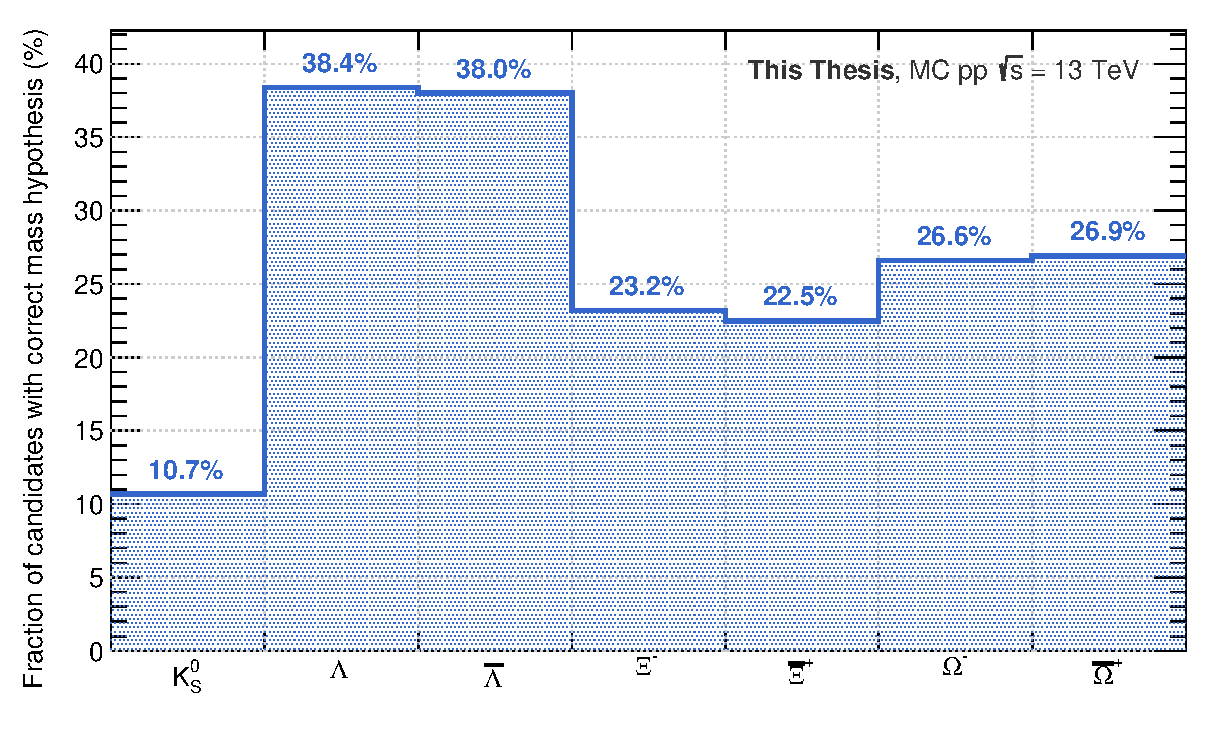
\includegraphics[width=1\textwidth]{Figs/Chapter5/FractionOfPIDForTracking.eps}
	\caption{Fraction de candidats V0s et cascades avec les hypothèses de masse adéquates sur l'ensemble de leurs produits de désintégration au cours de la reconstruction des traces.}
	\label{fig:FractionOfPIDForTracking}
\end{figure}

\item Dans le même esprit, la formule de Bethe-Bloch (\eq\ref{eq:BetheBloch}) dépend également de la particule traversant la détecteur, et plus spécifiquement de sa charge, son impulsion et sa masse. Ce dernier provient d'une mesure, au cours de la reconstruction des traces, du dépôt d'énergie dans la chambre à projection temporelle qui fournit une identification préliminaire des particules. Il n'y a, par contre, aucune garantie que celle-ci co\"incide avec l'hypothèse de masse attendue pour une désintégration d'un \rmKzeroS, \rmLambdaPM, \rmXiPM ou \rmOmegaPM. Par exemple, s'il y a une ambiguité, la masse du pion est prise comme valeur par défaut. En réalité, seule une fraction des candidats possèdent les hypothèses de masse adéquates sur l'ensemble des produits de désintégration, comme illustrée sur la \fig\ref{fig:FractionOfPIDForTracking}. Si l'hypothèse de masse considérée s'avère incorrecte, le calcul des pertes d'énergie sera erroné, menant finalement à un biais sur la masse measurée.

\end{enumerate}

Il existe différentes façons d'adresser ces problèmes. L'approche suivie dans cette analyse consiste à i) rejouer l'extrapolation des traces dans l'objectif de retirer les précédentes corrections des pertes d'énergie, puis ii) les ré-appliquer cette fois-ci en utilisant l'hypothèse de masse adéquate, les paramètres appropriés pour les matériaux du détecteur, et en arrêtant l'extrapolation à la position du vertex secondaire. Une partie conséquente de ce travail de thèse a consisté à implémenter cette procédure, dite de \textit{rétro-corrections}. La validité de cette procédure a été confirmée à l’aide de simulations Monte Carlo.

L'autre source dominante d'incertitudes systématiques a été déterminée par l'étude de la dépendance avec l'angle azimutal $\varphi$ de la masse mesurée. Il a été observé que cette dernière quantité varie fortement avec la direction transverse dans les données réelles  \fig\ref{fig:MassVsPhiACLambda}, tandis qu'elle est stable dans les simulations. Autrement dit, la tendance observée dans les données réelles n'est pas reproduites dans les simulations. Cela suggère que certains éléments de l'expérience ne sont pas pris en compte dans les productions Monte Carlo, comme par exemple de la matière non-comptabilisée ou des erreurs d'alignement résiduelles du trajectographe interne. Il s'avère que cette dépendance avec l'angle azimutal réduit drastiquement du côté~$z~>~0$ du détecteur. Ainsi l'origine de cette dépendance doit être trouvée du côté $z~<~0$ qui se distinguent par la présence d'un absorbeur à muons et d'un aimant dipolaire. Le premier est réputé pour être la source d'un grand nombre de particules secondaires, pouvant déformer la forme du bruit de fond et possiblement biaser la masse extraite. Cela est plutôt peu probable du fait des fortes purités en V0s et cascades. A l'inverse, l'aimant dipolaire a une influence sur le champ magnétique au sein du tonneau central. Les distortions induites ont d'ores et déjà été prises en compte dans la calibration du détecteur. Cependant, quelques distortions résiduelles peuvent toujours être présentes, affectant ainsi la trajectoire des particules et menant \textit{in fine} à une variation de la masse mesurée.

En résumé, l'origine de la dépendance azimutale ne peut pas être affirmée avec certitude. Il apparaît clairement que l'analyse devrait se concentrer du côté $z > 0$ du detecteur. Les variations residuelles de la masse mesurée, ne pouvant pas être englobées par les autres sources d'incertitudes systématiques, sont évaluées et prises comme incertitude systématique.\\

\begin{figure}[!t]
%\centering
\hspace*{-2.cm}
\subfigure[]{
	\includegraphics[width=0.65\textwidth]{Figs/Chapter5/MassLambda\_MomPhi\_ACsides\_MC.eps}
	\label{fig:MassVsPhiACMCLambda}
} 
\subfigure[]{
	\includegraphics[width=0.65\textwidth]{Figs/Chapter5/MassLambda\_MomPhi\_ACsides.eps}
	\label{fig:MassVsPhiACLambda}
} 
\caption{Masse mesurée des \rmLambda et \rmAlambda dans les collisions pp à \sqrtS = 13 \tev en fonction de la position azimutale du point de désintégration. Les résultats sur des données simulées sont présentés à gauche (a), ceux sur les données réelles à droite (b). Seules les incertitudes statistiques sont affichées.}
	\label{fig:MassVsACPhi}
\end{figure}


Les valeurs finales sur la masse des \rmXiPM et \rmOmegaPM sont :
\begin{align*}
    M(\rmXiM) &= 1321.968 \pm  0.025 \text{(stat.)} \pm 0.070 \text{(syst.)} \ \mmass ,\\
    M(\rmAxiP) &= 1321.918 \pm  0.025 \text{(stat.)} \pm 0.075 \text{(syst.)} \ \mmass ,\\
    M(\rmOmegaM) &= 1672.520 \pm  0.033 \text{(stat.)} \pm 0.102 \text{(syst.)} \ \mmass ,\\
    M(\rmAomegaP) &= 1672.571 \pm  0.033 \text{(stat.)} \pm 0.101 \text{(syst.)} \ \mmass.
\end{align*}

Les valeurs finales sur la différence de masse relative entre particule et anti-particule sont :

\begin{align*}
    2 \cdot \frac{M(\rmAxiP) - M(\rmXiM)}{M(\rmAxiP) + M(\rmXiM)} &= \left[ -3.34 \pm 2.67 \text{(stat.)} \pm 6.61 \text{(syst.)}\right] \times 10^{-5}\\
    &= \left[ -3.34 \pm 7.13 \text{(tot.)} \right] \times 10^{-5} ,\\
    \\
    2 \cdot \frac{M(\rmAomegaP) - M(\rmOmegaM)}{M(\rmAomegaP) + M(\rmOmegaM)} &= \left[ 3.44 \pm  3.00 \text{(stat.)} \pm 2.51 \text{(syst.)}\right ] \times 10^{-5}\\
    &= \left[ 3.44 \pm  3.92 \text{(tot.)} \right ] \times 10^{-5},
\end{align*} où l'incertitude totale est calculée en sommant quadratiquement les incertitudes statistiques et systématiques.

La précision finale sur la mesure de la masse est dominée par les incertitudes systématiques, et plus particulièrement celles liées à l'identification des candidats et à l'étalonnage du détecteur. Ces incertitudes comprennent la précision limitée du champ magnétique, la connaissance limitée de la quantité de matière, ainsi que les distortions résiduelles dans la calibration du détecteur qui entraînent des instabilités dans les résultats. Ce dernier facteur contribue également à l'incertitude statistique, étant donné que la principale approche pour garantir une mesure robuste a consisté à rejeter les candidats au lieu de les corriger. Par conséquent, la taille de l'incertitude statistique peut également être considérée comme une conséquence des distortions résiduelles. Ceci est particulièrement pertinent pour la différence de masse mesurée, puisque ces effets systématiques sur les valeurs de masse s'annulent dans la différence et ne se reflètent que dans l'incertitude statistique.

\`A propos, la première extraction de masse a permis d'estimer la quantité de baryons multi-étranges disponible dans notre échantillon de données : près de 2~500~000~\rmXi et environ 133~000~\rmOmega. En revanche, après application des sélections supplémentaires introduites tout au long de l'étude systématique, ces chiffres tombent à 16~373~$\pm$~133.3~\rmXiM et 15~611~$\pm$~130~\rmAxiP avec une pureté supérieure à 96\%, et 10~808~$\pm$~115~\rmOmegaM et 10~539~$\pm$~114~\rmAomegaP avec une pureté dépassant les 90\%. Bien que la mesure finale repose uniquement sur une fraction de l'échantillon de données de départ, les résultats actuels s'appuient toujours sur une statistique en baryons étranges bien plus grande que celles citées dans le PDG.\\


Par ailleurs, le méson \rmKzeroS et les hypérons \rmLambda ont également été utilisés comme valeurs de référence pour la mesure de la masse. Les valeurs finales sont :
\begin{align*}
    M\left(\rmKzeroS\right) &= 497.635 \pm  0.022 \text{(stat.)} \pm 0.256 \text{(syst.)} \ \mmass ,\\
    \\
    M\left(\rmLambda\right) &= 1115.752 \pm  0.011 \text{(stat.)} \pm 0.066 \text{(syst.)} \ \mmass ,\\
    M\left(\rmAlambda\right) &= 1115.799 \pm  0.010 \text{(stat.)} \pm 0.065 \text{(syst.)} \ \mmass.
\end{align*}
avec une différence de masse relative de\\
\begin{align*}
    2 \cdot \frac{M(\rmAlambda) - M(\rmLambda)}{M(\rmAlambda) + M(\rmLambda)} &= \left[ 3.91 \pm 1.34 \text{(stat.)} \pm 2.27 \text{(syst.)}\right] \times 10^{-5}\\
    &= \left[ 3.91 \pm 2.64 \text{(tot.)} \right] \times 10^{-5} .
\end{align*}

Les valeurs tabulées étant à $\mPDG(\rmKzeroS) = 497.611 \pm 0.013$ \mmass et \break\mbox{$\mPDG(\rmLambda) = 1115.683 \pm 0.006$ \mmass}, les masses mesurées des \rmKzeroS et \rmLambda sont en accord avec les valeurs de masse du PDG à environ $1 \sigma$. Cela est moins vrai pour les \rmAlambda, ce qui se reflète également dans la différence de masse relative entre particule et anti-particule\footnote{La différence de masse relative entre \rmLambda et \rmAlambda citée dans le PDG se situe à $\left(-0.1 \pm 1.1\right)\times 10^{-5}$.}. Cependant, l'accord reste raisonnablement bon.\\

Nos mesures pour les baryons multi-étranges doivent être comparées aux valeurs actuelles citées dans le PDG, ainsi que qu'aux mesures précédentes \figs\ref{fig:MassVsPDG}. Bien que l'incertitude sur les valeurs de masse des \rmOmegaPM a été réduite de plus d'un facteur deux, la précision sur la masse des \rmXiPM s'avère être au même niveau que l'incertitude tabulée dans les abaques internationaux. Cependant, notez que le PDG ne réalise pas de mesures de masse, mais fournit une valeur mondiale. Comme soulignés par les \figs\ref{fig:MassVsPDG}, nos mesures sont jusqu'à présent les plus précises dans le secteur des baryons multi-étranges, améliorant les précédentes \emph{mesures} d'environ un facteur 1.19 pour les \rmXiPM et 9.26 pour les \rmOmegaPM. Si l'on regarde les valeurs de masse, il semblerait que les résultats pour les \rmXiPM s'écartent des valeurs PDG de plus de $2\sigma$, ce qui pourrait indiquer un biais résiduel soit dans notre analyse, soit dans la mesure de masse précédente des \rmXiPM. 

\begin{figure}[!p]
%\centering
\hspace*{-2cm}
\subfigure[]{
	\includegraphics[width=0.6\textwidth]{Figs/Chapter5/MassXiMinus\_New.eps}
	\label{fig:MassXiMinusVsPDG}
} 
\subfigure[]{
	\includegraphics[width=0.6\textwidth]{Figs/Chapter5/MassXiPlus\_New.eps}
	\label{fig:MassXiPlusVsPDG}
}
\hspace*{-2cm}
\subfigure[]{
	\includegraphics[width=0.6\textwidth]{Figs/Chapter5/MassOmegaMinus\_New.eps}
	\label{fig:MassOmegaMinusVsPDG}
} 
\subfigure[]{
	\includegraphics[width=0.6\textwidth]{Figs/Chapter5/MassOmegaPlus\_New.eps}
	\label{fig:MassOmegaPlusVsPDG}
}
\caption{Comparaison de nos valeurs de masse pour les hypérons \rmXiM (a), \rmAxiP (b), \rmOmegaM (c) and \rmAomegaP (d), aux mesures précédentes citées dans le PDG en 2023 \cite{particledatagroupReviewParticlePhysics2022}. La ligne verticale et la zone grisée représentent la valeur PDG et l'incertitude associée respectivement.}
	\label{fig:MassVsPDG}
\end{figure}

\begin{figure}[!h]
%\centering
\hspace*{-2cm}
\subfigure[]{
	\includegraphics[width=0.6\textwidth]{Figs/Chapter5/MassDiff\_Xi\_New.eps}
	\label{fig:MassDiffXiVsPDG}
} 
\subfigure[]{
	\includegraphics[width=0.6\textwidth]{Figs/Chapter5/MassDiff\_Omega\_New.eps}
	\label{fig:MassDiffOmegaVsPDG}
}
\caption{Comparaison de nos valeurs de différence de masse entre les \rmXiM et \rmAxiP (a), et \rmOmegaM et \rmAomegaP (b), aux mesures précédentes citées dans le PDG en 2023 \cite{particledatagroupReviewParticlePhysics2022}. La ligne verticale et la zone grisée représente la valeur PDG et l'incertitude associée respectivement.}
	\label{fig:MassDiffVsPDG}
\end{figure}

En ce qui concerne les différences de masse relative (\figs\ref{fig:MassDiffVsPDG}), la précision a été améliorée d'un facteur de 1.20 pour les \rmXiPM et légèrement plus qu'un facteur deux pour les \rmOmegaPM. Au vue de leurs incertitudes, les valeurs sont compatibles avec zero, et en accord avec la symétrie CPT.



\chapter{Mesure de la production corrélée d'hadrons étranges}

Le QGP a fait l'objet d'études expérimentales depuis plus deux décennies maintenant, allant de l'annonce des premiers signes de son existence au SPS dans les années 2000 jusqu'à sa caractérisation fine au LHC aujourd'hui. Son exploration se fait via l'étude de ses signatures. Récemment, il a été observé que les petits systèmes de collisions présentent la plupart des signes habituellement attribués au QGP : corrélation à longue portée dans les collisions pp de plus faible multiplicité~\cite{alicecollaborationALICESeesRidge}, écoulement collectif \cite{cmscollaborationEvidenceCollectiveMultiparticle2015, alicecollaborationAnisotropicFlowFlow2023}, suppression des quarkonia lourds \cite{singhCharmoniumSuppressionUltrarelativistic2022}\footnote{Seuls les photons thermiques produit au sein du plasma et l'atténuation des gerbes hadroniques (\textit{jets}) n'ont pas (encore) été observés dans les petits systèmes, tandis qu'ils sont présents dans les collisions d'ions lourds. La recherche de ces deux signatures dans les petits systèmes sera davantage poursuivie lors des LHC Run-3 et Run-4 \cite{vanleeuwenHighlightsALICE59th2023}.}. Ces observations remettent en question les fondations mêmes du QGP : soit la vision de la physique du QGP doit être re-pensée et davantage ancrée sur les collisions pp, or inversement, la QCD dans les petits systèmes doit être étendue avec de nouveaux éléments pour introduire une collectivité semblable à celle observée dans les collisions d'ions lourds. D'une manière ou d'une autre, une meilleure description de la dynamique des collisions pp et d'ions lourds apparaît comme une nécessité absolue dans l'objectif de former \textit{in fine} un continuum de physique.

\begin{figure}[!p]
%\centering
\hspace*{-1.25cm}
\subfigure[]{
	\includegraphics[width=0.55\textwidth, valign=t]{Figs/Chapter6/img.jpg}
	\label{fig:PythiaVsStrangenessEnhancement}
} 
\subfigure[]{
	\includegraphics[width=0.6\textwidth, valign=t]{Figs/Chapter6/StrangenessEnhancement_CoreCorona.png}
	\label{fig:EposVsStrangenessEnhancement}
} 
\caption{Rapport des taux de production intégrés des hadrons étranges au pions en fonction de la multiplicité moyenne en particule chargée à rapidité centrale dans ALICE, comparé à différentes prédictions Monte Carlo. Sur la gauche, celui-ci est mesuré dans des collisions pp à \sqrtS = 7 et 13 \tev, p-Pb à \sqrtSnn = 5.02 \tev, Pb-Pb à \sqrtSnn = 2.76 \tev , et comparé à \Pythiaeight et \Herwig \cite{acharyaMultiplicityDependencePi2020} ; sur la droite, il s'agit de mesures en collisions pp à \sqrtS = 7 \tev et Pb-Pb à \sqrtSnn~=~2.76~\tev, avec différentes prédictions de \Epos \cite{wernerCorecoronaProcedureMicrocanonical2023}.}
	\label{fig:MCModelStrangenessEnhancement}
\end{figure}

L'une des principales signatures historiques du QGP est le renforcement de l'étrangeté, qui consiste en une augmentation de la production des hadrons multi-étranges dans les collisions d'ions lourds par rapport aux petits systèmes. Il a été observé que ces taux de production augmentent également de façon continu en allant des collisions pp de faible mutiplicité à celles de haute multiplicité. Différents modèles fondamentalement différents parviennent à reproduire qualitativement cette tendance (\fig\ref{fig:MCModelStrangenessEnhancement}). D'une part, il y a \Pythia \cite{bierlichComprehensiveGuidePhysics2022, skandsTuningPYTHIAMonash2014} qui modélise l'hadronisation des quarks à l'aide de cordes de Lund (\textit{Lund Strings}) ; ceux-ci correspondent à des champs de gluons qui se brisent lorsque l'énergie de tension de la corde est suffisament élevée, conduisant à la formation d'hadrons. Les dynamiques des collisions pp et d'ions lourds sont tous deux issues de l'interaction de ces cordes, c'est à comprendre que cette approche suppose l'absence d'un QGP. D'autre part, \Epos \cite{wernerCorecoronaProcedureMicrocanonical2023} repose nativement sur la diffusion multiple de partons, structurée selon une approche c\oe{}ur-couronne au sein de la collision : un c\oe{}ur dense accueillant un milieu collectif de type QGP, entouré d'une couronne de gaz hadronique \cite{wernerAnalysingRadialFlow2014}. Jusqu'à maintenant, aucune de ces deux approches n'a pu fournir une explication sans équivoque sur l'émergence des phénomènes collectifs dans les petits systèmes. Davantage de contraintes expérimentales sont nécessaires pour les distinguer et finalement identifier les mécanismes de production d'hadrons en jeu. \\

Une façon d'éclairer davantage la situation est de réaliser des études multi-différentielles, typiquement des corrélations angulaires et en rapidité entre différentes espèces d'hadrons. Ceux-ci apportent des informations sur la production des quarks, et de ce fait, sur leur hadronisation. Deux hadrons produits à partir de la brisure d'une corde de couleur en une paire de quark-antiquark, tel que modélisé par \Pythia, devrait montrer des signes d'une forte corrélation locale. En revanche, si les quarks sont produits au début de la collision -- les soi-disant \textit{pré-hadrons} dans le paradigme de \Epos \cite{wernerCorecoronaProcedureMicrocanonical2023} -- et s'hadronise plus tard, une telle corrélation devrait alors disparaître.

\begin{figure}[t]
\centering
%\hspace*{-1.25cm}
\includegraphics[width=0.8\textwidth]{Figs/Chapter6/PredictionPythia_Bierlich.png}
\caption{Prédictions de \Pythiaeight pour le rapport des taux de production des \rmOmega au \rmPiPM en fonction de la multiplicité en particule chargée dans les collisions pp à \sqrtS =  13 \tev, en présence d'une résonance \rmPhiMes (lignes en couleur) ou non (ligne noire). La configuration par défaut de \Pythia (\Pythiaeight, Monash 2013) est montrée en pointillés, tandis que les lignes pleines représentent le cas où les cordes de couleur (\textit{colour rope}) sont activées.}
	\label{fig:PredictionPythia_Bierlich}
\end{figure}

Un exemple d'une telle mesure nous provient des auteurs de \Pythia ; puisque l'étrangeté est conservée par l'interaction forte, le nombre d'hadrons étranges est censé être exactement compensé par le nombre d'hadrons anti-étranges, conduisant à une corrélation entre ces hadrons\footnote{Puisque tous les hadrons étranges sont corrélés entre eux, on peut contrôler, dans une certaine mesure, le contenu en étrangeté au sein de l'événement en ayant recours à un déclenchement sur une particule étrange, un \rmXi ou un \rmOmega par exemple.}. En particulier, au sein du paradigme classique des cordes de Lund, les baryons multi-étranges sont produits par la rupture d'une corde de couleur en une paire de diquark-antidiquark. Cependant, les développements récents visant à s'approcher des collisions d'ions lourds -- à savoir, la reconnexion de couleur et de cordes de couleur \cite{christiansenStringFormationLeading2015, bierlichEffectsOverlappingStrings2015a, adolfssonQCDChallengesPp2020} -- offrent de nouveaux mécanismes de production. En conséquence, il est attendu que i) l'abondance en \rmOmega augmente en présence d'un \rmPhiMes dans l'événement, et ii) cette augmentation devient plus importante à mesure que l'écart en rapidité entre les deux particules décroît (voir \fig\ref{fig:PredictionPythia_Bierlich}).

Jusqu'à présent, cette corrélation n'a jamais été mesurée. Une observable similaire a été étudiée récemment \cite{adolfssonStudyXiHadron2020}, qui analyse les corrélations angulaires entre le baryon multi-étrange \rmXiPM et un \pOrPbar, \rmPiPM, \rmKPM, \rmLambdaPM, \rmXiPM lui-même. Celle-ci n'a cependant pas été étendue au résonance \rmPhiMes, ni répétée avec les baryons \rmOmega. Cette analyse vise donc à vérifier cette prédiction en mesurant la production corrélée des \rmOmega et \rmPhiMes sur l'ensemble des collisions pp à une énergie dans le centre-de-masse de 13 \tev collectées tout au long du LHC Run-2 par ALICE. Dans le but de réduire autant que possible la contamination par le bruit de fond, une telle mesure nécessite un déclenchement avec une pureté très élevée, et donc d'une excellente capacité de contrôle sur la quantité de signal et de bruit de fond pour la particule de déclenchement. Pour cette raison et contrairement à la prédiction de \Pythia, la particule de déclenchement sera le \rmOmega et non pas le \rmPhiMes, la première offrant une pureté bien plus maîtrisable.

Puisque le baryon \rmXi est bien plus produit que le \rmOmega, deux mesures sont réalisées : d'abord, celle de la production corrélée des \rmXi et \rmPhiMes, puis celle des \rmOmega et \rmPhiMes. De cette façon, la faisabilité d'une telle mesure peut être testée sur les \rmXi, et le cas échéant, elle sera répétée avec les \rmOmega.\\

Par construction, ce type d'analyse s'appuient sur deux catégories de particules : les particules de déclenchement dites \textit{trigger}, qui sont ensuites corrélées avec les particules d'intérêts dans l'événement, les particules \textit{associées}. Dans la suite, le terme \textit{particule de déclenchement} renvoie soit à un baryon \rmXi ou \rmOmega, et la \textit{particule associée} correspond à la résonance \rmPhiMes. Ici, les baryons multi-étranges sont étudiés et sélectionnés de la même manière que dans la première analyse. Quant aux résonances \rmPhiMes, elles sont identifiés dans leur canal de désintégration  $\rmPhiMes \rightarrow \rmKPM \rmKMP $. Elles sont reconstruites par l’appariement de deux particules de charges électriques opposées. Du fait de leur faible temps de vie (\cTau = 46 \fmC), elles volent sur une très faible distance, rendant la position de désintégration indiscernable du vertex primaire. En conséquence, les combinaisons erronées ne peuvent pas être rejetées à l'aide de sélections géométriques. Pour réduire ce bruit de fond combinatoire, on recourt à une technique de mélange d'événements qui consiste à former des candidats \rmPhiMes par l'appariement de deux particules issus d'événements différents dans l'objectif de former intentionnellement des candidats erronées pour évaluer leur contribution et la retirer. 


Pour mesurer la corrélation entre un baryon multi-étrange -- soit \rmXiPM ou \rmOmegaPM -- et un méson \rmPhiMes, ces deux particules sont associées par paires et l'on étudie comment la population des paires de particules se distribuent selon une variable donnée. Plus précisément, ici on se concentre sur production corrélée des \rmPhiMes dans les événements contenant, au moins, un baryon multi-étrange. Ainsi, l'observable d'intérêt est le taux de production des mésons \rmPhiMes par particules de déclenchement en fonction de leur écart en rapidité $\Delta y$ et en azimut $\Delta \varphi$,
\begin{align}
\frac{1}{N_{\text{trigger}}} \cdot \dNXdX{pairs}{$y$} (\Delta y) &= \frac{1}{\dNXdy{cascade}} \cdot \dNXdXdy{pairs}{$\Delta y$},\\
\frac{1}{N_{\text{trigger}}} \cdot \dNXdX{pairs}{$y$} (\Delta \varphi) &= \frac{1}{\dNXdy{cascade}} \cdot \dNXdXdy{pairs}{$\Delta \varphi$}.
\end{align}
où $N_{\text{pairs}}$ correspond au nombre de paires cascade-\rmPhiMes.

Il s'ensuit une série de corrections visant à compenser l'inefficacité de reconstruction des résonances et l'acceptance limitée du detecteur ALICE, ainsi qu'à retirer autant que possible la contribution du bruit de fond et des paires non-corrélées. Une étude préliminaire des biais systématiques a également été réalisée ; seules les sources attendues comme les sources les plus naturelles, et probablement dominantes, d'incertitudes systématiques sont retenues : l'identification des baryons multi-étranges et des mésons \rmPhiMes. Cette étude préliminaire des biais systématiques permet de se faire une idée de l'incertitude totale sur notre mesure et ouvre la porte vers une première interprétation des résultats.\\

\afterpage{
\begin{landscape}
\begin{figure}[!p]
%	\hspace{-2.cm}
\vspace*{-1cm}
%\centering
\subfigure[]
	{
	\includegraphics[width=0.8\textwidth, angle=0]{Figs/Chapter6/FinalPerTriggerYield\_VsRap\_XiPhi\_Ratio\_MBAndHM.eps}
	\label{fig:FinalPerTriggerYieldXiRapMBAndHM}
	}
\subfigure[]
	{
	\includegraphics[width=0.8\textwidth, angle=0]{Figs/Chapter6/FinalPerTriggerYield\_VsRap\_XiPhi\_Ratio\_PythiaAndEPOS.eps}
	\label{fig:FinalPerTriggerYieldXiRapPythiaAndEPOS}
	}\\
%\centering
\subfigure[]
	{
	\includegraphics[width=0.8\textwidth, angle=0]{Figs/Chapter6/FinalPerTriggerYield\_VsPhi\_XiPhi\_Ratio\_MBAndHM.eps}
	\label{fig:FinalPerTriggerYieldXiPhiMBAndHM}
	}
\subfigure[]
	{
	\includegraphics[width=0.8\textwidth, angle=0]{Figs/Chapter6/FinalPerTriggerYield\_VsPhi\_XiPhi\_Ratio\_PythiaAndEPOS.eps}
	\label{fig:FinalPerTriggerYieldXiPhiPythiaAndEPOS}
	}
\caption{\`A gauche : mesures finales de la corrélation entre les hypérons \rmXiPM et les résonances \rmPhiMes, aux rapidités centrales ($\absrap < 0.5$), en fonction de (a) leur différence en rapidité, $\Delta y$, et (c) en azimut, $\Delta \varphi$, dans les collisions pp de biais minimum (marqueur plein) et de haute multiplicité (marqueur vide) à \sqrtS = 13 \tev. \`A droite : comparaison à différentes prédictions Monte Carlo (\Pythiaeight Monash 2013, \Pythiaeight avec les mécanismes de reconnexion de couleur et de cordes de couleur, \EposFour avec une paramétrisation simple de l'évolution hydrodynamique) pour la corrélation en (b) $\Delta y$ et (d) $\Delta \varphi$ pour les collisions pp à \sqrtS = 13 \tev de biais minimum. Les barres d'erreurs comprennent les incertitudes statistiques et systématiques.}
	\label{fig:FinalPerTriggerYieldXi}
\end{figure}
\end{landscape}

\begin{figure}[!p]
%	\hspace{-2.cm}
\centering
\subfigure[]
	{
	\includegraphics[width=1\textwidth, angle=0]{Figs/Chapter6/FinalPerTriggerYield\_VsRap\_OmegaPhi\_Ratio\_HM.eps}
	\label{fig:FinalPerTriggerYieldOmegaRapMBAndHM}
	}
\centering
\subfigure[]
	{
	\includegraphics[width=1\textwidth, angle=0]{Figs/Chapter6/FinalPerTriggerYield\_VsPhi\_OmegaPhi\_Ratio\_HM.eps}
	\label{fig:FinalPerTriggerYieldOmegaPhiMBAndHM}
	}
\caption{Mesures finales de la corrélation entre les hypérons \rmOmegaPM et les résonances \rmPhiMes, aux rapidités centrales ($\absrap < 0.5$), en fonction de (a) leur diff	\'erence en rapidité, $\Delta y$, et (b) en azimut, $\Delta \varphi$, dans les collisions pp de haute multiplicité à \sqrtS = 13 \tev. Les barres d'erreurs comprennent les incertitudes statistiques et systématiques.}
	\label{fig:FinalPerTriggerYieldOmega}
\end{figure}
}

Les mesures finales des taux de production des \rmPhiMes par particules \textit{trigger} dans les collisions pp de biais minimum et de haute multiplicité à une énergie dans le centre-de-masse de 13 \tev sont présentées dans les \figs\ref{fig:FinalPerTriggerYieldXi} et \ref{fig:FinalPerTriggerYieldOmega} avec un \rmXiPM et \rmOmegaPM comme particule de déclenchement respectivement.

Le taux de production des \rmPhiMes par particules de déclenchement dans les données de bias minimum sur la \fig\ref{fig:FinalPerTriggerYieldXiRapMBAndHM} est compatible avec l'unité sur l'ensemble de la plage en rapidité. Par conséquent, aucune corrélation entre la production des \rmXiPM et des \rmPhiMes n'est observée en $\Delta y$. En revanche, la \fig\ref{fig:FinalPerTriggerYieldXiPhiMBAndHM} présente une corrélation azimutale : lorsque le \rmPhiMes est produit à une faible distance angulaire d'un baryon \rmXiPM, son taux de production augmente d'environ 35\%.

Les résultats dans les événements de haute multiplicité suivent les mêmes tendances : pas de corrélation avec la séparation en rapidité, alors qu'il y en a une avec la distance en azimut. Cependant, les dépendances en $\Delta y$ et $\Delta \varphi$ sont moins marquées, avec une augmentation de la production des résonances \rmPhiMes atteignant au mieux les 15\%. Cela suggère que leur production est moins dépendante, moins liée à celle d'un \rmXiPM dans les collisions pp de haute multiplicité, et que les \rmPhiMes peuvent être produits via d'autres processus.\\

En raison de la statistique limitée des données de biais minimum, la production corrélée d'hadrons étranges en présence d'un baryon \rmOmegaPM ne peut, pour le moment, qu'être étudiée dans les événements de multiplicité élévée. Compte tenu des incertitudes sur la \fig\ref{fig:FinalPerTriggerYieldOmegaRapMBAndHM}, aucune corrélation \rmOmegaPM-\rmPhiMes avec la différence en rapidité n'est observable. La \fig\ref{fig:FinalPerTriggerYieldOmegaPhiMBAndHM} montre un signe d'une augmentation de la production des \rmPhiMes lorsqu'ils sont produits proche en azimut d'un baryon triplement étrange. Toutefois, il est difficile de tirer des conclusions définitives avec la précision actuelle.\\


Pour mieux comprendre les mécanismes d'hadronisation en jeu ici, une comparaison entre nos mesures expérimentales et les prédictions théoriques est nécessaire. Cette comparaison s'articule principalement autour de deux modèles\break phénoménologiques: d'une part, il y a \Pythiaeight avec la configuration par défault, Monash 2013, ou celle incluant les mécanismes liées à la reconnexion de couleur et aux cordes de couleur (\textit{Colour Rope}, CR) ; d'autre part, il y a \EposFour avec sa décomposition c\oe{}ur-couronne (\textit{core-corona}). Ici, on exploite une version rapide de \EposFour qui recourt à une paramétrisation relativement simple de l'évolution hydrodynamique du c\oe{}ur -- appelé \textit{parametrised fluid expansion} (PFE) -- afin d'accélérer la génération d'événements Monte Carlo\footnote{La génération de 100 collisions proton-proton avec \EposFour avec PFE prend environ 1 minute. \`A titre de comparaison, cela prend approximativement 2 heures et 45 minutes en modélisant complétement l'évolution hydrodynamique du c\oe{}ur.}. Au total, 1,3 milliards de collisions pp à \sqrtS = 13 \tev ont été générées avec \Pythiaeight dans sa configuration Monash 2013 et dans la configuration des cordes de couleur\footnote{Strictement parlant, il n'existe de version officielle de \Pythia incluant les mécanismes liés à la reconnexion de couleur et aux cordes de couleur. La configuration la plus proche à une telle version peut être trouvée en annexe dans la version complète du manuscrit.}, et 600 millions d'événements pp avec une énergie dans le centre-de-masse de 13 \tev avec \EposFour en utilisant la PFE.

La comparison aux différents modèles a été réalisée à l'aide de \Rivet (\textit{Robust Independent Validation of Experiment and Theory}) \cite{hepforgeRivetParticlephysicsMC2023}. Le \tab\ref{tab:SummaryCorrelatedProductionStatus} donne une vue d'ensemble de l'état actuel de l'analyse. Jusqu'à présent, la comparaison aux données Monte Carlo se concentre sur les événements de bias minimum. Puisque la corrélation \rmOmegaPM-\rmPhiMes peut seulement être mesurée dans les collisions pp à haute multiplicité avec les données du LHC Run-2, aucune étude comparative des mesures et des prédictions Monte Carlo ne peut être faite dans le cas présent.

La \fig\ref{fig:FinalPerTriggerYieldXiRapPythiaAndEPOS} montre que l'ensemble des prédictions considérées reproduisent qualitativement bien l'évolution avec $\Delta y$. La précision expérimentale ne permet cependant pas de distinguer les différents modèles. En ce qui concerne la corrélation \rmXiPM-\rmPhiMes avec la séparation azimutale (\fig\ref{fig:FinalPerTriggerYieldXiPhiPythiaAndEPOS}), \Pythiaeight Monash 2013, \Pythiaeight avec les mécanismes CR et \EposFour avec PFE présentent la même tendance. Plus précisément, ils fournissent tous une description similaire des régions transverse et opposée de la distribution, et sont qualitativement en accord avec les mesures. Par contre, les deux \say{configurations} de \Pythiaeight surestiment le taux de production dans la région à forte proximité azimutale ($\Delta \varphi \sim 0$) tandis que \EposFour le sous-estime. Cette différence peut être interprétée comme une conséquence des caractéristiques propres à chacun des modèles : la fragmentation des cordes de Lund dans \Pythiaeight correspond au processus d'hadronisation dominant dans les processus durs, alors que \EposFour fournit également une description des processus plus doux via l'hydrodynamique au sein du c\oe{}ur. Il est intéressant de noter qu'il n'y a aucune différence significative entre les prédictions de \Pythiaeight Monash 2013 et \Pythiaeight CR. Ainsi, l'augmentation de l'abondance des \rmPhiMes en présence d'un \rmXiPM ne peut être pas être décrite par des mécanismes uniquement associées à des processus durs, et repose au moins partiellement sur une composante plutôt douce.\\


\begin{table}[t]
%    \centering
\hspace*{-2cm}
    \begin{tabular}{c|c|c|c|c|c}
    \noalign{\smallskip}\hline \noalign{\smallskip}
    \bf \bf Type de & \bf \'Echantillon & \bf Mesure de la & \multicolumn{3}{c}{\bf Comparaison aux modèles MC}\\
    \bf corrélation & \bf de données & \bf corrélation & \Pythiaeight \textsc{Monash 2013} & \Pythiaeight \textsc{Colour Rope} & \EposFour\\
    \noalign{\smallskip}\hline \noalign{\smallskip}
    \multirow{2}*{\rmXiPM-\rmPhiMes} & MB & \CheckGr & \CheckGr & \CheckGr & \CheckGr \\
     & HM & \CheckGr & \ToDo & \ToDo & \ToDo \\
    \noalign{\smallskip}\hline \noalign{\smallskip}
    \multirow{2}*{\rmOmegaPM-\rmPhiMes} & MB & \NoWay & \CheckGr & \CheckGr & \CheckGr \\
     & HM & \CheckGr & \ToDo & \ToDo & \ToDo \\
    \noalign{\smallskip}\hline \noalign{\smallskip}
    \end{tabular}
    \caption{\'Etat actuel de l'analyse sur la production corrélée des baryons multi-étranges et des résonances \rmPhiMes dans les collisions proton-proton à \sqrtS = 13 \tev. Le symbole \CheckGr indique que celui-ci a déjà été fait, \ToDo signifie qu'il doit être fait et \NoWay veut dire que cela ne peut pas être avec les données du LHC Run-2.}
    \label{tab:SummaryCorrelatedProductionStatus}
\end{table}

Une telle étude bénéficierait largement d'une comparaison des modèles avec les résultats à haute multiplicité, en particulier pour ceux impliquant les baryons \rmOmegaPM comme particules de déclenchement. L'analyse sera poussée dans cette direction dans les semaines à venir.

Par ailleurs, cette analyse pourrait être affinée et améliorée, notamment en ce qui concerne les baryons \rmOmegaPM. La statistique disponible étant le facteur limitant, même dans collisions pp à haute multiplicité, cela n'est réalisable qu'à l'aide des données du LHC Run-3. \`A titre de comparaison, au cours de l'année 2022, trois cents fois plus de données que dans le LHC Run-2 ont été enregistrées \cite{cern152ndLHCCMeeting2022}. Outre cette énorme quantité de données, ALICE met actuellement en \oe{}uvre un déclenchement sur la présence d'un candidat cascade reconstruit, conçu typiquement pour le type d'analyse ici présentée. 

Malgré les limites statistiques des données du LHC Run-2, cette analyse a montré le potentiel d'une telle mesure de corrélation, qui pourra prendre toute son ampleur dans un avenir proche avec les données du LHC Run-3.


\chapter{Conclusion}


Au début de ces trois années de doctorat, en 2020, le LHC était au milieu de sa seconde longue période d'arrêt. Pour une expérience installée sur le collisionneur tel que ALICE, il s'agit d'un moment décisif : l'expérience doit mener à bien son programme de rénovation et d'amélioration du détecteur à temps pour le début du LHC Run-3, et simultanément, elle doit finaliser les analyses de physique de la précédente campagne de prise de données. La présente thèse contribue à ce dernier point. En particulier, elle propose de pousser l'analyse de données jusqu'aux limites de ce qui est possible avec ALICE pendant le LHC Run-2 en effectuant des mesures de précision dans le secteur des saveures légères, avec des baryons multi-étranges. \`A cet égard, deux analyses ont été effectuées.\\


\begin{table}[h]
    \hspace{-1.3cm}
    \begin{tabular}{cccc|ccc}

%    \begin{tabular}{b{2cm}@{\hspace{0.5cm}} b{3cm}@{\hspace{0.5cm}} b{2cm}@{\hspace{0.5cm}} b{2cm}@{\hspace{0.5cm}} b{5cm}@{\hspace{0.5cm}} b{3cm}@{\hspace{0.5cm}} b{3cm}@{\hspace{0.5cm}}}
    \noalign{\smallskip}\hline \noalign{\smallskip}
    \bf Particule & \bf Masse & \multicolumn{2}{c|}{\bf Incertitude} & \bf Précédente & \multicolumn{2}{c}{\bf Incertitude}\\
    & \bf mesuré & \bf stat. & \bf syst. & \bf mesure de masse & \bf stat. & \bf syst.\\
    & (\mmass) & (\mmass) & (\mmass) & (\mass) & (\mmass) & (\mass) \\
    \noalign{\smallskip}\hline \noalign{\smallskip}
    \rmXiM & 1321.968 & 0.025 & 0.070 & 1321.70 & 0.08 & 0.05 \\
	\rmAxiP & 1321.918 & 0.025 & 0.075 & 1321.73 & 0.08 & 0.05 \\
    \noalign{\smallskip}\hline \noalign{\smallskip}
    \rmOmegaM & 1672.520 & 0.033 & 0.102 & 1673 & \multicolumn{2}{c}{1} \\ 
    \rmAomegaP & 1672.571 & 0.033 & 0.101 & 1673 & \multicolumn{2}{c}{1} \\ 
	\noalign{\smallskip}\hline \noalign{\smallskip}
	\bf Particule & \bf Différence de & \multicolumn{2}{c|}{\bf Incertitude} & \bf Précédente & \multicolumn{2}{c}{\bf Incertitude}\\
    & \bf mass mesurée & \bf stat. & \bf syst. & \bf différence de masse & \multicolumn{2}{c}{\bf totale} \\
    & ($\times 10^{-5}$) & ($\times 10^{-5}$) & ($\times 10^{-5}$) & ($\times 10^{-5}$) & \multicolumn{2}{c}{($\times 10^{-5}$)}\\
    \noalign{\smallskip}\hline \noalign{\smallskip}
    \rmXi & -3.34 & 2.67 & 6.61 & 2.5 & \multicolumn{2}{c}{8.7} \\
    \noalign{\smallskip}\hline \noalign{\smallskip}
    \rmOmega & 3.44 & 3.00 & 2.51 & 1.44 & \multicolumn{2}{c}{7.98}\\ 
	\noalign{\smallskip}\hline \noalign{\smallskip}
    \end{tabular}
    \caption{\`A gauche : les mesures finales de masse et de différence de masse relative pour les \rmXiPM et \rmOmegaPM, avec leurs incertitudes statistiques et systématiques. \`A droite : les précédentes mesures de masse et de différence de masse relative pour les \rmXiPM \cite{abdallahMassesLifetimesProduction2006} et \rmOmegaPM \cite{hartouniNclusiveRoductionEnsuremath1985, chanMeasurementPropertiesOverline1998}, avec leurs incertitudes statistiques et systématiques. Si ces valeurs ne sont pas précisées dans la publication, l'incertitude totale est indiquée.}\label{tab:FinalResultsCPT}
\end{table}

La première mesure de cette thèse consiste en une mesure précise de la masse des \rmXiM, \rmAxiP, \rmOmegaM, \rmAomegaP et des différences de masse entre particule et anti-particule. Le point de départ de cette analyse est l'observation que les dernières mesures de ce type datent d'il y a 17 et 25 ans, et reposent sur une faible statistique. En comparaison, la présente mesure tire parti des excellentes capacités de reconstruction de ALICE au cours du LHC Run-2, et de la production abondante d'hadrons étranges dans les collisions pp à une énergie dans le centre-de-masse de 13 \tev : environ 2~500~000~$(\rmXiM + \rmAxiP)$ et approximativement 133~000~$(\rmOmegaM + \rmAomegaP)$.  

Il a été montré qu'une compréhension fine de la reconstruction des données est nécessaire pour réaliser une telle mesure, et rapidement les limites de la calibration du détecteur sont atteintes. Pour surmonter ces limitations, une importante fraction de la statistique a dû être sacrifiée. Les mesures finales -- présentées dans le \tab\ref{tab:FinalResultsCPT} -- peuvent tout de même rivaliser avec les dernières mesures citées dans le PDG, et les améliorent d'un facteur 1.20 et 2 pour la différence de masse relative des baryons \rmXi et \rmOmega respectivement. Au vue de leur précision, les deux résultats sont en accord avec l'invariance de la symétrie CPT. Les résultats présentés ici sont en cours de finalisation, et devraient donner lieu à une publication dans le futur. Un \textit{Analysis Review Committee} a déjà été formé ; une première version d'une note d'analyse ALICE a déjà été examinée.\\

%\begin{figure}[h]
%%\centering
%\hspace*{-2cm}
%\subfigure[]{
%	\includegraphics[width=0.6\textwidth]{Figs/Chapter5/MassDiff\_Xi\_New.eps}
%	\label{fig:MassDiffXiVsPDGFinal}
%} 
%\subfigure[]{
%	\includegraphics[width=0.6\textwidth]{Figs/Chapter5/MassDiff\_Omega\_New.eps}
%	\label{fig:MassDiffOmegaVsPDGFinal}
%}
%\caption{Comparison of our mass difference values between the \rmXiM and \rmAxiP (a), and the \rmOmegaM and \rmAomegaP, to the past measurements quoted in the PDG, as of 2023 \cite{particledatagroupReviewParticlePhysics2022}. The vertical line and the shaded area represent the PDG average and its associated uncertainty.}
%	\label{fig:MassDiffVsPDGFinal}
%\end{figure}

\`A partir de cette première analyse, ce travail de thèse se poursuit avec une seconde visant à étendre l'étude des baryons multi-étranges vers la compréhension de leur mécanismes de production dans les collisions pp aux énergies du LHC. En particulier, nous voulons comprendre comment l'étrangeté se distribue dans l'événement et idéalement suivre le flux de quarks étranges. \`A cette fin, l'idée est de corréler les particules produites : que ce soit entre particules étranges et non-étranges ($\rmLambdaPM - \proton$, $\rmLambdaPM - \rmPiPM$, etc) ou entre hadrons étranges. Ces derniers recouvrent différents types de corrélations : baryon-méson ($\Lambda [uds] - \rmKzeroS [d\bar{s}]$, etc) ou baryon-baryon ($\rmXiM [dss] - \rmAlambda [\bar{u}\bar{d}\bar{s}]$, $\rmXiM[dss] - \rmAxiP [\bar{d}\bar{s}\bar{s}]$, $\rmOmegaM[sss] - \rmAomegaP [\bar{s}\bar{s}\bar{s}]$, etc). Dans tous les cas, cela demande de mesurer la corrélation entre deux particules \textit{identifiées}.

Parmi l'ensemble des possibilités, nous avons mis en place une tâche d'analyse dans le but d'étudier les corrélations entre des baryons multi-étranges -- soit un \rmXiPM ou un \rmOmegaPM\ -- et un \pOrPbar, \rmPiPM, \rmKPM, \rmKstarZero, \rmKzeroS, \rmLambdaPM, \rmXiPM, \rmOmegaPM. En pratique, l'analyse se concentre spécifiquement sur la corrélation d'un baryon multi-étrange avec une résonance \rmPhiMes. Une telle mesure s'avère plutôt difficile : le but est de corréler deux particules \textit{identifiées}, avec des taux de production relativement faibles\footnote{Sur un millier d'événements, on peut s'attendre approximativement à 38 \rmPhiMes, 20 \rmXi et 2~\rmOmega à rapidité centrale ($\absrap < 0.5$) dans les collisions pp à \sqrtS = 13 \tev \cite{alicecollaborationProductionLightflavorHadrons2021}. De plus, ils doivent appartenir au même événement pour être considérés dans l'analyse.}. Alors que la première analyse vise une haute pureté, celle-ci recherche plutôt une haute efficacité de sélection.

Cette contrainte expérimentale est importante pour distinguer entre différents modèles phénoménologiques. Par exemple, la configuration \textit{Monash 2013} de \Pythia prédit une augmentation de l'abondance des \rmOmega en présence d'un \rmPhiMes dans l'événement qui décroît avec la multiplicité en particule chargée, tandis que la configuration comprenant la reconnexion de couleur et les cordes de couleur anticipe un accroissement avec la multiplicité. 

Les résultats préliminaires liés à cette corrélation indiquent que la statistique disponible en baryons \rmOmega et résonances \rmPhiMes restent trop faible dans les collisions~pp de biais minimum ; en ce qui concerne les hypérons \rmXi, les corrélations angulaire et en rapidité ont été étudiées séparément. Aucune structure dans la corrélation dépendant de la rapidité ne peut être observée pour le moment, alors qu'une corrélation azimutale apparaît. Pour mieux comprendre les mécanismes en jeu, une comparaison entre nos mesures expérimentales et les prédictions de différents modèles MC a été effectuée. Cet aspect a été réalisé en se concentrant principalement sur \Pythia et \EposFour. Celle-ci suggère que la production corrélée des baryons \rmXiPM et des résonances \rmPhiMes dans les collisions pp de biais minimum consiste vraisemblablement en une combinaison de mécanismes d'hadronisation doux et durs.

L'analysis a également été étendue aux collisions proton-proton de haute multiplicité. La même tendance que dans les données de biais minimum peut être observée, bien que la corrélation semble moins prononcée, ce qui suggére que la production des \rmPhiMes est également réalisée via d'autres mécanismes n'impliquant pas la production d'un hypéron \rmXiPM. Concernant la corrélation \rmOmegaPM-\rmPhiMes, aucune dépendance avec la séparation en rapidité ne peut être identifiée alors qu'une peut l'être avec l'écart en azimut. Cependant, en raison des limitations statistiques, aucune conclusion définitive ne peut être tirée.\\

Ces deux mesures mettent en perspective les limites du détecteur ALICE durant le LHC Run-2. D'une part, les incertitudes sur les valeurs de masse et différence de masse sont dominées par la calibration du détecteur. En particulier, la source dominante de biais systématiques provient des distortions résiduelles. Pour les maintenir sous contrôle, une partie importante des données a dû être rejetée, entraînant dans des incertitudes plus élevées. D'autre part, la second mesure souffre d'un manque de statistique, ce qui empêche de tirer des conclusions définitives. La solution à ces limitations peut certainement être trouvée avec le LHC Run-3.

La collaboration ALICE a mené un important programme de rénovation et d'amélioration du dispositif expérimental au cours de la seconde longue période d'arrêt du LHC (2018-2022) avec deux objectifs principaux : améliorer la résolution spatiale du système de trajectographie, et augmenter la cadence de prise de données. Grâce à ces améliorations, sur l'ensemble de la prise de données de 2022, l'expérience a enregistré environ 35 \invpb de collisions pp à \sqrtS~=~13.6~\tev \cite{cern152ndLHCCMeeting2022}. En comparaison, la luminosité inspectée sur l'ensemble des collisions pp dits de biais minimum (\textit{minimum bias}) du LHC Run-2 s'élève à 0.059 \invpb, et jusqu'à 13 \invpb pour les collisions de plus haute multiplicité. En d'autres termes, sur une période d'un an, la statistique disponible a été multipliée par un facteur 300.

Cependant, cette performance a un coût : pour atteindre de telles capacités de prise de données, certains détecteurs doivent être poussés à leurs limites, ce qui entraîne des instabilités. En particulier, à de tels taux d'interaction, les ions dans le volume gaseux de la chambre à projection temporelle (\textit{{\bf T}ime {\bf P}rojection {\bf C}hamber}, TPC) commencent à s'accumuler sous la forme d'une charge d'espace, créant des distortions dans le champ électro-statique et déteriorant ainsi les performances de trajectographie. Cet effect de charge d'espace peut être corrigé en appliquant la calibration appropriée. La TPC étant le principal trajectographe, la clé de la prise de données de ALICE tourne autour du contrôle des distortions dûes aux charges d'espace. Ainsi, comme dans la première analyse, tout le défi consiste à dériver une calibration précise. Bien que la calibration actuelle de la TPC soit loin d'être suffisante pour améliorer ces analyses avec les données du LHC Run-3, ALICE est sortie de la seconde longue période d'arrêt en tant qu'une nouvelle expérience. Les performances globales continuent de s'améliorer, et il est à espérer que, dans les mois à venir, une calibration potentiellement meilleure que celle du LHC Run-2 sera disponible. 

De plus, le système de trajectographie interne (\textit{{\bf I}nner {\bf T}racking {\bf S}ystem}, ITS) a été remplacé par un nouveau trajectographe, l'ITS-2, avec une meilleure résolution spatiale et un budget de matière réduit. Afin d'améliorer la calibration globale du détecteur ALICE, une partie de la thèse a été consacrée au pré-alignement de l'ITS-2. Il s'agit d'une étape critique dans la mise en service du detecteur, puisqu'il sert de point de départ pour l'alignement final du dispositif. L'alignement global et actuel du détecteur ALICE a été réalisé à la fin 2022, en utilisant les paramètres de pré-alignement identifiés au cours de ce travail de thèse.

En opération dans les collisions pp durant les prises de données en 2022 et 2023, le détecteur ITS-2 se révèle robuste avec typiquement 98-99\% des capteurs ALPIDE opérationels \cite{alicecollaborationALICEUpgradesLHC2023}. La grande disponibilité, couplée à une haute efficacité de détection par couche, limitent considérablement les pertes dans l'acceptance des détecteurs.\\

%Furthermore, in view of improving the overall calibration of the ALICE detector, a fraction of the thesis has been dedicated to the pre-alignment of the ITS-2 detector. This is critical stage in the commissionning of the detector, as it acts as input for the final alignment of the apparatus. The current global alignment of the ALICE detector have been performed at the end of 2022, using the pre-alignment parameters identified during this PhD.
%
%Moreover, the ITS has been replaced with a new Inner Tracking System, the ITS-2, with a better spatial resolution and a reduced material budget. In operation in pp collisions in 2022 and 2023, the ITS-2 detector proves to be robust with typically 98-99\% of ALPIDE sensors that are operational \cite{alicecollaborationALICEUpgradesLHC2023}. The high availability, coupled with the high detection efficiency per layer limit drastically the losses in the acceptance of the detectors.\\

De façon similaire aux mesures réalisées tout au long de ce travail de thèse, le LHC Run-3 a son lot de défis à relever. Il offre en retour une reconstruction des traces améliorée, une meilleure calibration du détecteur et une quantité prodigieuse de données. Compte tenu des limitations mises en lumière dans cette thèse, les prochaines mesures de précision ne pourront qu'être réalisées avec cette version améliorée de ALICE. Bien qu'il reste encore du chemin à parcourir, une chose est sûre : l'ère de précision est droit devant. 